% 依固定题面中正方体的点线关系重绘；投影不表示长度、角度比例。
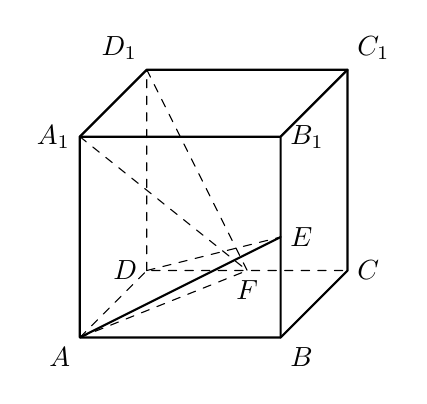
\begin{tikzpicture}[scale=0.85,line join=round,line cap=round]
\coordinate (A) at (0,0);
\coordinate (B) at (3,0);
\coordinate (C) at (4,1);
\coordinate (D) at (1,1);
\coordinate (Aone) at (0,3);
\coordinate (Bone) at (3,3);
\coordinate (Cone) at (4,4);
\coordinate (Done) at (1,4);
\coordinate (E) at (3,1.5);
\coordinate (F) at (2.5,1);
\draw[thick] (A)--(B)--(C)--(Cone)--(Done)--(Aone)--cycle;
\draw[thick] (Aone)--(Bone)--(Cone) (B)--(Bone);
\draw[dashed] (A)--(D)--(C) (D)--(Done);
\draw[thick] (A)--(E);
\draw[dashed] (D)--(E) (A)--(F) (Aone)--(F) (Done)--(F);
\node[below left] at (A) {$A$};
\node[below right] at (B) {$B$};
\node[right] at (C) {$C$};
\node[left] at (D) {$D$};
\node[left] at (Aone) {$A_1$};
\node[right] at (Bone) {$B_1$};
\node[above right] at (Cone) {$C_1$};
\node[above left] at (Done) {$D_1$};
\node[right] at (E) {$E$};
\node[below] at (F) {$F$};
\end{tikzpicture}
